\chapter{Definizione del problema}
\setcounter{section}{1}

(replicazione dei dati - introduzione)
\subsection{Cluster di database}
\subsection{Rete di pari}
\subsection{Sistemi di ridondanza disco (RAID)}
\subsection{Codice di correzione errore (erasure coding)}
\section{Hardware utilizzato per gli esperimenti}
\section{Software utilizzato per gli esperimenti}

\subsection{PG Logical}
PG Logical \`e un sistema logico di replica implementato come estensione di PostgreSQL. Completamente integrato, non richiede alcun triggers o programmi esterni. Questa alternativa alla replica fisica \`e un metodo altamente efficiente per replicare i dati utilizzando un modello di publish/subscribe per la replica selettiva.

I vantaggi offerti da Pg Logical sono i seguenti:
\begin{itemize}
\item
Replica sincrona
\item
Replica ritardata
\item
Risoluzione dei conflitti configurabili
\item
Capacit\`{a} di convertire lo standby fisico in una replica logica
\item
Pu\`{o} pubblicare i dati da PostgreSQL a un abbonato Postgres-XL
\item
Le sequenze possono essere replicate
\item
Nessun trigger significa ridurre il carico di scrittura sul Provider
\item
Nessuna re-esecuzione di SQL significa overhead e latenza ridotti per il Sottoscrittore
\item
Il sottoscrittore non \`{e} in ripristino di riposo caldo, in modo da poter utilizzare tavoli temp, non sbloccati o normali
\item
Non \`{e} necessario annullare le query per consentire alla replica di continuare la riproduzione
\item
Il sottoscrittore (Subscriber) pu\`{o} avere diversi utenti e protezione, indici diversi, impostazioni di parametri diversi
\item
Replica solo un database o un sottoinsieme di tabelle, noto come set di replica (Replication Sets)
\item
Replicare in versioni o architetture di PostgreSQL, consentendo aggiornamenti a bassa o zero-downtime
\item
Pi\`{u} server a monte in un singolo subscriber per l'accumulo di cambiamenti
\end{itemize}

Casi di uso:
I diagrammi che seguono descrivono i gestori di database delle funzioni che sono in grado di eseguire con PgLogical.
\begin{figure}[htbp]
\centering
Migrare e aggiornare PostgreSQL con tempi di inattivit\`a quasi a zero
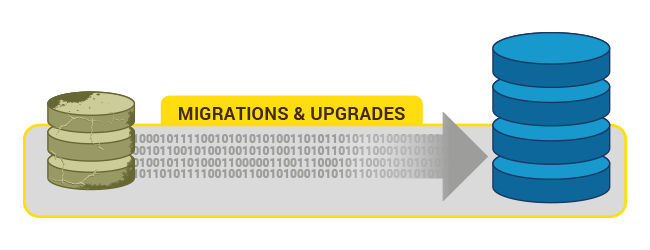
\includegraphics[scale=0.70]{img/pglogical_1.png}\\
\caption{Migrazione e aggiornamenti PostgreSQL \label{figura1} \cite{etichetta1}}
Accumulare le modifiche provenienti da server di database scartati in un data warehouse
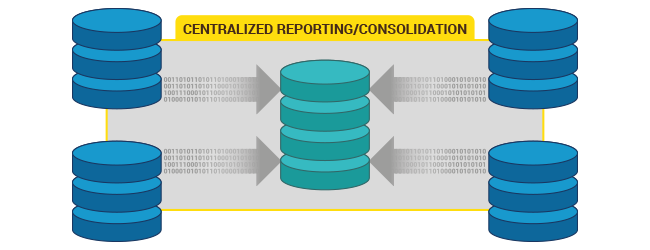
\includegraphics[scale=0.70]{img/pglogical_2.png}\\
\caption{Aggregazione \label{figura2} 
\cite{etichetta2}}
\end{figure}
\begin{figure}[htbp]
\centering
Copiare tutti o una selezione di tabelle di database ad altri nodi di un cluster
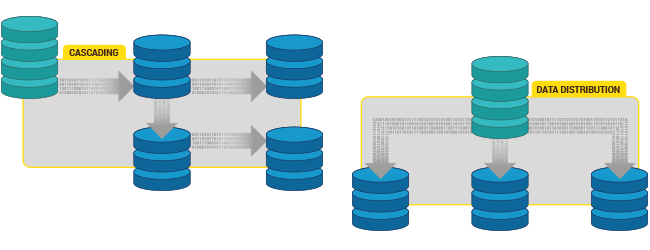
\includegraphics[scale=0.70]{img/pglogical_3.png}\\
\caption{A cascata e distribuzione dati \label{figura3} \cite{etichetta2}}
Le modifiche del database in tempo reale ad altri sistemi
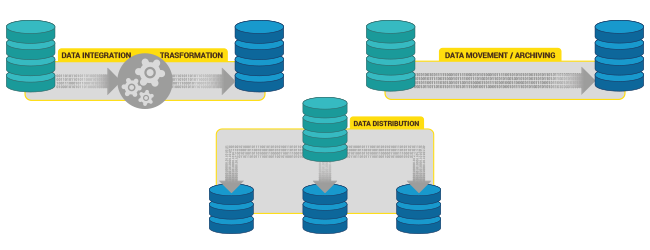
\includegraphics[scale=0.70]{img/pglogical_4.png}\\
\caption{A cascata e distribuzione dati \label{figura4} \cite{etichetta2}}
\end{figure}
